% Descripción de la SRCNN
\subsection{Red Neuronal Convolucional de Super Resolución: (SRCNN por sus siglas en inglés)}
Como se menciona en \cite{freeman}, tradicionalmente se utilizan 3 etapas para la super resolución de imagenes:
\begin{enumerate}
    \item Extracción de parches en baja resolución y representación en un vector de "alta" dimensión
    \item Mapeo entre vectores (parches de baja resolución) de baja resolución con vectores que representan parches de alta
    resolución
    \item Reconstrucción de imagén
\end{enumerate}
Estas 3 etapas generalmente se realizan por separado, es por ello que se propone el uso de una red convolucional en la cual se
lleven a cabo estas 3 operaciones de manera conjunta.\\
En \cite{SRCNN} se propone una red convolucional que consté de 3 capas, cada una correspondiente a las etapas que clasicamente
se siguen para el problema de super resolución, es decir, 1) Se diseña una primer capa convolucional con la cual se busca la
"extracción" de los parches de baja resolución, 2) una capa que estará conectada directamente con la salida de la primer capa
convolucional, y que será la encargada de realizar el "mapeo" entre los parches de baja resolución y los parches de alta
resolución y 3) una capa final encargada de realizar la reconstrucción de la imagen de alta resolución.

\begin{figure}[H]
    \label{fig:SRCNN_Arquitectura}
    \centering
    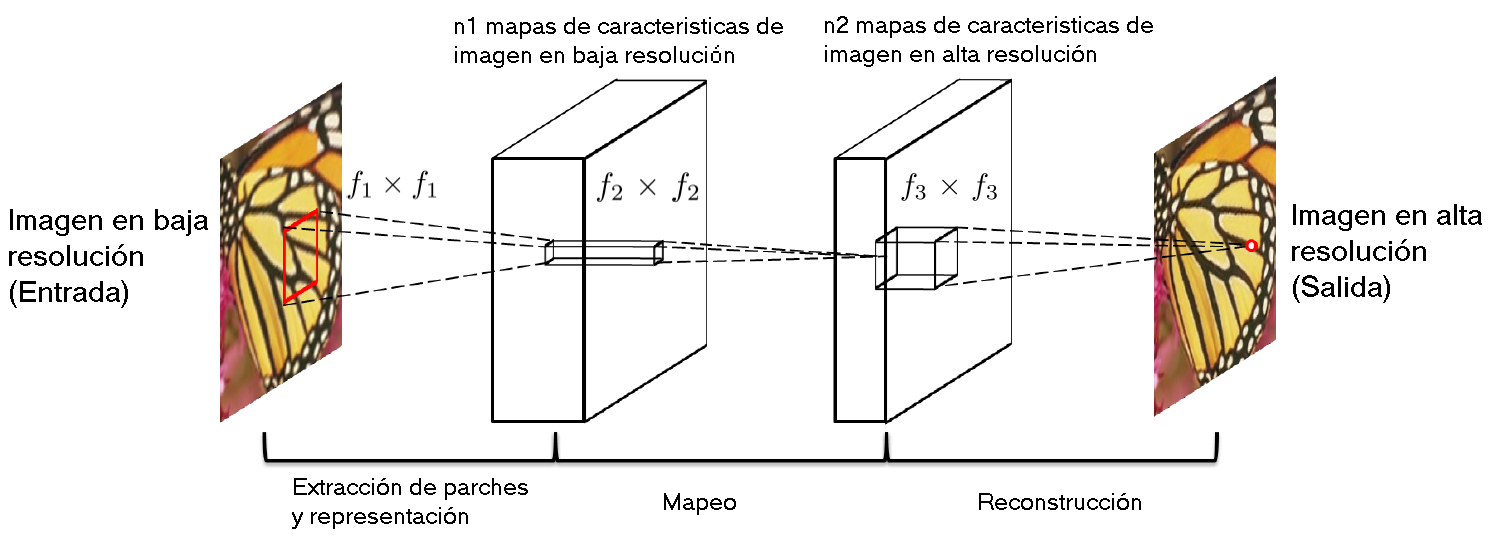
\includegraphics[scale = 0.6]{SRCNN_Arquitectura.png}
    \caption{Arquitectura de la SRCNN}
\end{figure}

Se busca generar un mapeo directo entre la imagen de baja resolución (Y) y la de alta resolución real (X).

\textbf{1. Extracción de parches}\\
Esta etapa comunmente se basa en la extracción de parches de baja resolución y representarlos por un conjunto de bases pre-entrenadas
tales como PCA,DCT,Haar,etc. Esto es equivalente a "convolucionar" la imagen por un conjunto de filtros, donde cada uno de estos
representaria las bases pre-entrenadas. En la formulación de la SRCNN, se envuelve la optimización de estas bases en la optimización
de la red. Formalmente, la primer capa se expresa como una operación $F_1$:
\begin{align}
    \label{eqn:SRCNN_FirstLayer}
    F_1(Y)=max(0,W_1*Y+B_1)
\end{align}
Donde $Y$ y $B_1$ representan los filtros y el \emph{bias} respectivamente y el operador "$*$" denota la operación de convolución.
Se utiliza la función de activación \textbf{ReLU} (ReLU,$max(0,x)$) en las respuestas de los filtros.\\

\textbf{2. Mapeo}\\
La primer capa extrae caracteristicas de $n_1$ dimensiones para cada parche. En la segunda operación se realiza un mapeo de cada
uno de estos vectores de dimensiones $n_1$ con vectores de dimensiones $n_2$. Esto es equivalente a aplicar $n_2$ filtros. Esta
descripción es válida para filtros de kernel $1\times1$, pero es facil generalizar para otros tamaños de \emph{kernel}, solo que
ahora el mapeo se realiza en parches de kernel $p\times p$. La operación de la segunda capa es:

\begin{align}
    \label{eqn:SRCNN_SecondLayer}
    F_2(Y)=max(0,W_2*F_1(Y)+B_2)
\end{align}

Cada uno de los vectores de salida de dimensiones $n_2$ es conceptualmente la reprsentación de un parche en alta resolución que
será utilizado para la reconstrucción.\\

\textbf{3. Reconstrucción}\\
En los métodos tradicionales, la predicción de traslapamiento de parches de alta resolución es frecuentemente promediada para
producir la imagen final. El promediado puede ser considerado como un filtro pre-definido sobre un conjunto de mapas de
características (Donde cada posición es la forma de vector "aplando" de un parche de alta resolución). Se define una capa
convolucional para producir la imagen final en alta resolución:

\begin{align}
    \label{eqn:SRCNN_ThirdLayer}
    F(Y)=W_3*F_2(Y)+B_3
\end{align}